\documentclass{report}
\usepackage[a4paper, total={7in, 10.3in}]{geometry}
\usepackage[fleqn]{amsmath}
\usepackage{amssymb}
\usepackage{amsthm}
\usepackage{enumitem}
\usepackage[]{mdframed}
\usepackage{multicol}
\usepackage{thmtools}
\usepackage{graphicx}
\usepackage{tikz}
\usepackage{tipa}
\usepackage{mathtools}
\usepackage{titletoc,tocloft}
\usepackage{ifxetex}
\usepackage{setspace}
\usepackage{array, makecell, cellspace}
\setlength{\cellspacetoplimit}{13.2ex}
\setlength{\cellspacebottomlimit}{13.2ex}
\ifxetex
      \usepackage{substitutefont}
      \substitutefont{T3}{\rmdefault}{cmr}
\fi
\title{Calculus}
\author{Melvin Chia}
\newcommand{\sol}[1]{
      \noindent \textbf{Sol.}
}
\newcommand{\prooff}[1]{
      \noindent \textbf{Proof.}
}
\newcommand{\arc}[1]{{%
                  \setbox9=\hbox{#1}%
                  \ooalign{\resizebox{\wd9}{\height}{\texttoptiebar{\phantom{A}}}\cr#1}}}
\DeclareRobustCommand\iff{\ \Longleftrightarrow\ }
\DeclarePairedDelimiterX{\set}[1]{\{}{\}}{\setargs{#1}}
\NewDocumentCommand{\setargs}{>{\SplitArgument{1}{;}}m}
{\setargsaux#1}
\NewDocumentCommand{\setargsaux}{mm}
{\IfNoValueTF{#2}{#1} {#1\,\delimsize|\,\mathopen{}#2}}%{#1\:;\:#2}
\def\eos{\quad\hbox{\rlap{\hbox{\vrule depth 1.5pt height 2.6mm width 0.2mm \hskip 1mm \vrule height 2.6mm width 0.2mm}}{\vbox{\hrule height 0.2mm width 1.4mm \vskip 2.8mm \hrule depth 1.5pt height -0.35mm width 1.2mm}}}}
\counterwithout{equation}{chapter}
\setlength{\columnseprule}{1pt}
\setlength{\columnsep}{24pt}
\hfuzz=100pt
\mdfdefinestyle{MyFrame}{%
      linecolor=black,
      linewidth=1pt,
      roundcorner=20pt,
      innertopmargin=12pt, innerbottommargin=12pt, innerrightmargin=12pt,
      innerleftmargin=12pt, leftmargin = 4pt, rightmargin = 4pt, skipbelow=12pt,
      %backgroundcolor=gray!50!white}
}
\begin{document}
\maketitle
\onehalfspacing
\tableofcontents
\chapter{Limits}
\begin{multicols}{2}
      \begin{enumerate}
            \item $\lim\limits_{x \to 3}3x$
            \item $\lim\limits_{x \to -1}(x^2 + 4x)$
            \item $\lim\limits_{x \to 3}(9 - x^2)$
            \item $\lim\limits_{n\to-2}(x^{2}-2x+1)$
            \item $\lim\limits_{x\to-4}x^{2}(x+2)$
            \item $\lim\limits_{h\to2}(h^{2}\ -4h+4)$
            \item $\lim\limits_{a\to-1}(a+3)\left(a-4\right)$
            \item $\lim\limits_{x\to3}{\dfrac{x^{2}-5}{x+2}}$
            \item $\lim\limits_{x\to-2}{\dfrac{x^{3}+8}{x+2}}$
            \item $\lim\limits_{x\to4}\dfrac{x^2-5x+6}{x-3}$
            \item $\lim\limits_{x\to3}{\dfrac{3x}{x+2}}$
            \item $\lim\limits_{x\to5}{\dfrac{x-5}{2x^{2}-9x-5}}$
            \item $\lim\limits_{x\to1}{\dfrac{x-1}{x^{2}+x-2}}$
            \item $\lim\limits_{x\to4}{\dfrac{x-1}{x^{2}+x-2}}$
            \item $\lim\limits_{x\to-2}{\dfrac{x-2}{x^{2}-4}}$
            \item $\lim\limits_{h\to0}{\dfrac{2x^{2}h\ +3h}{h}}$
            \item $\lim\limits_{h\to0}\dfrac{{(2+h)}^{2}-4}{h}$
            \item $\lim\limits_{h\to0}{\dfrac{{(1+h)}^{3}-1}{h}}$
            \item $\lim\limits_{x\to-1}2x(x^{2}-4)$
            \item $\lim\limits_{x\to3}{\dfrac{x^{2}+2}{x+1}}$
            \item $\lim\limits_{x\to2}\left(x^{2}-3x+5\right)$
            \item $\lim\limits_{x\to1}{\dfrac{2x^{2}+1}{3x^{2}+4x-1}}$
            \item $\lim\limits_{x\to1}{\dfrac{x^{2}-5x+6}{x^{2}-9}}$
            \item $\lim\limits_{x\to-1}{\dfrac{x^{3}+1}{x+1}}$
            \item $\lim\limits_{x\to1}{\dfrac{x^{3}-1}{x-1}}$
            \item $\lim\limits_{x\to0}{\dfrac{2x^{3}+3x^{2}}{x^{3}}}$
            \item $\lim\limits_{k\to0}{\dfrac{{(x-k)}^{2}-2k x^{3}}{x(x+k)}}$
            \item $\lim\limits_{x\to1}{\dfrac{x^{2}-2x+5}{x^{2}+7}}$
            \item $\lim\limits_{x\to-2}{\dfrac{x^{4}-16}{x^{3}-2}}$
            \item $\lim\limits_{x\to1}{\dfrac{x-1}{x^{2}-1}}$
            \item $\lim\limits_{x\to0}{\dfrac{{\sqrt{1+x}}-1}{x}}$
            \item $\lim\limits_{x\to2}{\dfrac{x^{2}+4}{x^{2}+1}}$
            \item $\lim\limits_{x\to0}{\dfrac{x^{2}+3x+2}{x^{2}+2}}$
            \item $\lim\limits_{x\to1}{\dfrac{x^{2}-2x+1}{x^{2}\ -1}}$
            \item $\lim\limits_{x\to1{}}(3x^{2}-6x+5)$
            \item $\lim\limits_{x\to1}{\dfrac{2x^{2}-1}{3x^{3}-6x^{2}+5}}$
            \item $\lim\limits_{x\to1}{\dfrac{x^{2}-1}{x^{2}-4x+3}}$
            \item $\lim\limits_{x\to3}{\dfrac{x^{2}-\,5x+6}{7x^{2}-22x+3}}$
            \item $\lim\limits_{x\to3}{\dfrac{x^{3}-2x^{2}-2x+4}{x^{3}+x^{2}-10x+8}}$
            \item $\lim\limits_{x\to1}{\dfrac{x^{4}+2x^{2}-3}{x^{2}-3x+2}}$
            \item $\lim\limits_{x\to1}{\dfrac{1-{\sqrt[4]{x}}}{1-{\sqrt[3]{x}}}}$
            \item $\lim\limits_{x\to0}{\dfrac{\sqrt[n]{1+x}-1}{x}} \quad (n \in \mathbb{W})$
            \item $\lim\limits_{x\to1}{\dfrac{2-{\sqrt{x+3}}}{x^{2}-1}}$
            \item $\lim\limits_{x\to16}{\dfrac{\sqrt[4]{x}-2}{\sqrt{x}-4}}$
            \item $\lim\limits_{x\to2}(x^{2}+3x-1)$
            \item $\lim\limits_{x\to{-1}}{\dfrac{x^{2}+2}{x^{2}+x+3}}$
            \item $\lim\limits_{x\to{-1}}{\dfrac{x^{3}+1}{x^{2}-1}}$
            \item $\lim\limits_{x\to1}{\dfrac{x^{5}-x^{4}}{x^{3}-x}}$
            \item $\lim\limits_{x\to a}{\dfrac{x^{2}+a x-2a^{2}}{x^{2}-a^{2}}},a\neq0$
            \item $\lim\limits_{x\to a}{\dfrac{\sqrt{3x-a}-{\sqrt{x+a}}}{x-a}}$
            \item Given that $f(x) = x^2 - 3x$, find $\lim\limits_{h\to0}\dfrac{f(x+h)-f(x)}{h}$
            \item $\lim\limits_{x\to2}{\sqrt{2x^{2}+1}}$
            \item $\lim\limits_{x\to7}\dfrac{x^{2}\sqrt{x+2}}{x^{2}+14}$
            \item $\lim\limits_{x\to0}{\dfrac{{\sqrt{3x+4}-2}}{x}}$
            \item $\lim\limits_{x\to0}{\dfrac{1}{x^{2}}}$
            \item $\lim\limits_{x\to1}{\dfrac{1}{x-1}}$
            \item $\lim\limits_{x\to1}{\dfrac{4x-3}{x^{2}-5x+4}}$
            \item $\lim\limits_{x\to\infty}{\dfrac{3x^{3}-4x^{2}+2}{7x^{3}+5x^{2}-3}}$
            \item $\lim\limits_{n\to\infty}x^{2}$
            \item $\lim\limits_{x\to\infty}{\dfrac{3x^{2}-2x-1}{2x^{3}-x^{2}+5}}$
            \item $\lim\limits_{n\to\infty}\dfrac{1}{n^{2}}(1+2+3+\cdots+n)$
            \item $\lim\limits_{n\to\infty}\left[{\dfrac{1+2+3+\cdots+n}{n+2}}-{\dfrac{n}{2}}\right]$
            \item $\lim\limits_{n\to\infty}\left[{\dfrac{1}{1\cdot2}}+{\dfrac{1}{2\cdot3}}+\cdot\cdot\cdot+{\dfrac{1}{n(n+1)}}\right]$
            \item $\lim\limits_{x\to\infty}{\dfrac{5x^{3}+4x^{2}-6x+2}{8x^{3}-7x^{2}+4x-1}}$
            \item $\lim\limits_{x\to\infty}{\dfrac{x^{4}-2x^{3}+x^{2}+3}{x^{5}-x^{4}+1}}$
            \item $\lim\limits_{x\to\infty}{\dfrac{x^{3}-8x^{2}+4x-1}{x^{2}-6x+3}}$
            \item $\lim\limits_{x\to\infty}(\sqrt{x^{4}+1}-x^{2})$
            \item Find $\lim\limits_{n \to \infty}a_n$ of the following:
                  \begin{enumerate}
                        \item $a_{n}=1-{\dfrac{1}{n^{2}}}$
                        \item $a_{n}={\dfrac{4n-3}{8+6n}}$
                        \item $\lim\limits_{n \to \infty}\sum\limits_{k=1}^{n}\dfrac{k^2}{n^3}$
                        \item $a_{n}=\dfrac{n+2n^{2}+3n^{3}}{4n^{3}-7}$
                        \item $a_{n}={\dfrac{1+2+3+\cdots+n}{n^{2}}}$
                  \end{enumerate}
            \item Let $a_{n}={\left(\dfrac{{(-1)}^{n+1}}{\sqrt[3]{n^{2}+1}}\right)}\dfrac{1}{n}$,
                  find $\lim\limits_{n \to \infty}a_n$.
            \item $\lim\limits_{n\to\infty}\sqrt{4+{\left({\dfrac{1}{n}}\right)}^{2}}$
            \item $\lim\limits_{n\to\infty}{\left(\dfrac{n!}{n^{n}}\right)}$
            \item $\lim\limits_{n\to\infty}{\dfrac{4^{n}}{n!}}$
            \item Given $\vert\dfrac{f(x)-f(c\,)}{x-c}\vert\,\leq M,\ \forall x\not=c$
            \item If $\vert f(x)\vert \le B$ for all $x$, show that
                  $\lim\limits_{x\to0}\,x^{2}f(x)=0$
            \item $\lim\limits_{x\to\infty}\left(\dfrac{1}{\sqrt{n^{2}+1}}+\cdots+\dfrac{1}{\sqrt{n^{2}+2}}+\cdots+\dfrac{1}{\sqrt{n^{2}+n}}\right)$
            \item Given $a > b > 0$, find
                  $\lim\limits_{n\to\infty}{\left(a^{n}+b^{n}\right)}^{\frac{1}{n}}$
            \item $\lim\limits_{n\to\infty}\dfrac{\vert-1+h\vert-\vert-1\vert}{h}$
            \item $\lim\limits_{n\to\infty}\dfrac{3^n + 2^n}{3^n}$
            \item $\lim\limits_{n\to\infty}\dfrac{4^{n}+1}{4^{n}}$
            \item $\lim\limits_{n\to\infty}{\dfrac{1-3^{n}}{3^{n}}}$
            \item Find $\lim\limits_{n\to\infty}a_n$ of the following:
                  \begin{enumerate}
                        \item $a_n = 3^{n}+3^{-n}$
                        \item $a_n = {(\sqrt{3})}^n2^{-n}$
                        \item $a_n = \dfrac{5^{1-n}}{6^{1-n}}$
                        \item $a_n = (2\sin45^\circ\cos45^\circ)$
                        \item $a_n = {\dfrac{{(-1)}^{n}}{2n^{2}}+1}$
                        \item $a_n = \dfrac{1}{n}\left[n+{(-1)}^n\right]$
                  \end{enumerate}
            \item $\lim\limits_{x\to\infty}{\dfrac{1-x^{2n}}{1+x^{2n}}} \quad (x \in \mathbb{R})$
            \item Find $\lim\limits_{n\to\infty}a_n$ of the following:
                  \begin{enumerate}
                        \item $a_n = \dfrac{1}{n}{(\cos60^\circ)}^{n}$
                        \item $a_n = {\left(\dfrac{1}{2}\right)}^n\cos nx$
                        \item $a_n = 2^n - 2^{-n}$
                        \item $a_n = {(\sin^2 30^\circ + \cos^2 30^\circ)}^n$
                  \end{enumerate}
            \item $\lim\limits_{n\to\infty}(\sqrt{n^2 + n} - n)$
            \item $\lim\limits_{n\to\infty}(\sqrt{n^2 - 2n} - n)$
            \item $\lim\limits_{n\to\infty}(\sqrt{n+1} - \sqrt{n})$
            \item $\lim\limits_{x\to\infty}(\sqrt{x+\sqrt{x+\sqrt{x}}} - \sqrt{x})$
            \item $\lim\limits_{t\to2}\dfrac{\sqrt{1+\sqrt{2+t}}-\sqrt{3}}{t-2}$
            \item $\lim\limits_{x\to1}\left(\dfrac{1}{1-x} - \dfrac{3}{1-x^3}\right)$
            \item $\lim\limits_{x\to1}{\dfrac{12x^{11}-12x}{4x(x^{2}-1)}}$
            \item $\lim\limits_{x\to5}\left[\left(\dfrac{1}{x}-\dfrac{1}{5}\right)\left(\dfrac{1}{x-5}\right)\right]$
            \item $\lim\limits_{x\to2}\left(\dfrac{1}{x^2-x-2} - \dfrac{1}{2x^2-5x+2}\right)$
            \item $\lim\limits_{x\to0}{\dfrac{1}{x}}\left[{\dfrac{1}{(x+2)^{2}}}-{\dfrac{1}{4}}\right]$
            \item $\lim\limits_{x\to1}\left({\dfrac{x^{3}-1}{x^{2}-1}}-{\dfrac{x-{\dfrac{1}{x}}}{x-1}}\right)$
            \item $\lim\limits_{x\to 1}\left(\dfrac{1}{x-1}-\dfrac{2}{x^{2}-1}\right)$
            \item $\lim\limits_{x\to-\infty}{\dfrac{\sqrt{x^{2}+x+1}}{x+3}}$
            \item $\lim\limits_{x\to-2}\left(\dfrac{x}{x-1}+\dfrac{x^{2}+3x+2}{x^{2}-4}\right)$
            \item $\lim\limits_{x\to6}(\dfrac{2x-17}{x^{2}-7x+6}+\dfrac{x-5}{x-6})$
            \item $\lim\limits_{x\to-\infty}\dfrac{\sqrt[146]{x}}{\sqrt[7]{10^7}+\sqrt[3]{10^3}+\sqrt[7]{x+10^7}}$
            \item $\lim\limits_{x\to-\infty}{\dfrac{\sqrt{\dfrac{9x^{2}+1}{x+4}}}{x+4}}$
            \item $\lim\limits_{x\rightarrow-\infty}\dfrac{x\sqrt{-x}}{\sqrt{1-4x^{3}}}$
            \item $\lim\limits_{n\rightarrow\infty}{\dfrac{\sqrt[3]{\dfrac{x^{3}+x+4}{4}}}{1+x}}$
            \item $\lim\limits_{n\to4}\dfrac{\sqrt{x+5}-3}{x-4}$
            \item $\lim\limits_{x\to-8}\dfrac{\sqrt{1-x}-3}{2+\sqrt[3]{x}}$
            \item $\lim\limits_{x\to0}\dfrac{\sqrt{x+5}-\sqrt{5}}{2x}$
            \item $\lim\limits_{x\rightarrow0}\dfrac{\sqrt{9+x}-\sqrt{9-x}}{x}$
            \item $\lim\limits_{x\to4}{\dfrac{{\sqrt{x+5}}-3}{x-4}}$
            \item $\lim\limits_{x\to0}{\dfrac{{\sqrt{x+4}}-2}{x}}$
            \item $\lim\limits_{t\to0}{\dfrac{9-t}{3-{\sqrt{t}}}}$
            \item $\lim\limits_{x\to2}\dfrac{\sqrt{x+7}-3}{\sqrt{x+2}-2}$
            \item $\lim\limits_{x\to a}\dfrac{\dfrac{1}{\sqrt{x}}-\dfrac{1}{\sqrt{a}}}{x-a}$
            \item $\lim\limits_{h\to0}{\dfrac{{\sqrt[3]{a+h}}-\sqrt[3]{a-h}}{h}} \quad (a\neq0)$
            \item $\lim\limits_{t\to0}{\dfrac{\sqrt{1+t}-1}{t}}$
            \item $\lim\limits_{h\to0}{\dfrac{\sqrt{x+h}-\sqrt{x}}{h}}$
            \item $\lim\limits_{x\to0}\dfrac{1}{x}(\sqrt{1+x+x^{2}}-1)$
            \item $\lim\limits_{x\to2}\dfrac{\sqrt{1+\sqrt{2+x}}-\sqrt{3}}{x-2}$
            \item $\lim\limits_{x\to0}\dfrac{\sqrt{1+x^2}-\left(1+\dfrac{x}{2}\right)}{x^2}$
            \item $\lim\limits_{x\rightarrow2}\left(\dfrac{1}{x^{2}-4}-\dfrac{\sqrt{x-1}}{x^{2}-4}\right)$
            \item $\lim\limits_{x\rightarrow\infty}\dfrac{\sqrt[3]{8+x+x^{3}}-\sqrt[3]{8+x}}{\sqrt[3]{8+x}-\sqrt[3]{8+x^{3}}}$
            \item $\lim\limits_{x\to\infty}({\sqrt{x^{2}+1}}-x)$
            \item $\lim\limits_{x\to0}\dfrac{\sqrt{2+x}-\sqrt{3x-2}}{\sqrt{4x+1}-\sqrt{5x-1}}$
            \item $\lim\limits_{x\to\infty}(\sqrt{x^2+1}-\sqrt{x^2-4x})$
            \item $\lim\limits_{x\to\infty}(\sqrt{x^2+x-1}-\sqrt{x^2-x})$
            \item $\lim\limits_{x\to\infty}(\sqrt{x^2+x}-x)$
            \item $\lim\limits_{x\rightarrow27}{\dfrac{\sqrt{1+\sqrt[3]{x}}-2}{x-27}}$
            \item $\lim\limits_{x\to\infty}(\sqrt{x^2+9}-x)$
            \item $\lim\limits_{x\to\infty}\sqrt{x}(\sqrt{x+a}-\sqrt{x+b})$
            \item $\lim\limits_{x\to\infty}(\sqrt{x^2+x}-\sqrt{x^2+10})$
            \item Find the value of each of the following.
            \item $\lim\limits_{x\to1}(x-1)$
            \item $\lim\limits_{x\to1}{\dfrac{x^{2}-2}{x}}$
            \item $\lim\limits_{x\to0}{\dfrac{2x-5}{x+3}}$
            \item $\lim\limits_{x\rightarrow a}(x-a)$
            \item $\lim\limits_{x\to0}{\dfrac{2x^{2}-5x}{x}}$
            \item $\lim\limits_{x\to2}{\dfrac{x^{2}-4}{x-2}}$
            \item $\lim\limits_{x\to5}{\dfrac{x^{2}+4x-45}{x-5}}$
            \item $\lim\limits_{x\to1}{\dfrac{\log_{\mathrm{10}}x^{2}}{\log_{\mathrm{10}}x}}$
            \item $\lim\limits_{x\to9}{\dfrac{x-9}{\sqrt{x}-3}}$
            \item $\lim\limits_{x\to-1}{\dfrac{x+1}{\sqrt{x+5}-2}}$
            \item $\lim\limits_{x\to9}{\dfrac{\sqrt{x+7}-4}{x-9}}$
            \item $\lim\limits_{x\to2}{\dfrac{\sqrt{6-x}-2}{3-{\sqrt{11-x}}}}$
            \item The following diagram shows part of a graph $y = f(x)$.
                  \begin{center}
                        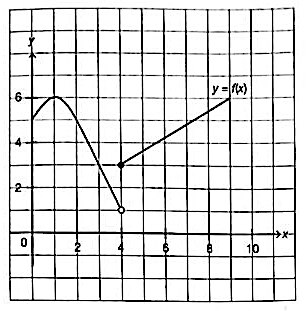
\includegraphics[width=0.4\textwidth]{./images/q4.jpeg}
                  \end{center}
                  Based on this graph, find
                  \begin{enumerate}
                        \item $f(4)$
                        \item $\lim\limits_{x\to4}{f(x)}$ and explain your answer.
                              Since the left limit and right limit are different, $f(4)$ does not exist.
                        \item $\lim\limits_{x\to1}{f(x)}$
                  \end{enumerate}
      \end{enumerate}
\end{multicols}
\chapter{Differentiation}
\begin{multicols}{2}
      \section{The First Derivative}
      \begin{enumerate}
            \item Find the first derivative for each of the following functions.
                  \begin{enumerate}
                        \item $y = 6x^2$
                        \item $y = -x^4$
                        \item $y = \sqrt[3]{x^4}$
                        \item $y = -\dfrac{2}{x^2}$
                  \end{enumerate}
            \item Find each of the following.
                  \begin{enumerate}
                        \item ${\dfrac{d}{d x}}\Big(2x^{2}+3x-9{\Big)}$
                        \item ${\dfrac{d}{d x}}\left(x^{2}+{\dfrac{2}{x}}\right)$
                        \item ${\dfrac{d}{d x}}\left(5x^{3}+2x^{2}+4x-7-{\dfrac{1}{x}}+{\dfrac{3}{x^{2}}}\right)$
                  \end{enumerate}
            \item Differentiate each of the following functions with respect to x.
                  \begin{enumerate}
                        \item $f(x)=x\left({\dfrac{1}{2}}x^{4}-x^{2}-5x\right)$
                        \item $f(x)=(x^{2}-5)(x+3)$
                        \item $f(x)={\dfrac{(x^{3}-x+4)}{x}}$
                        \item $f(x)={\dfrac{(x^{2}-x-2)}{(x-2)}}$
                  \end{enumerate}
            \item Find $f'(x)$ for each of the following functions.
                  \begin{enumerate}
                        \item $f(x)={(3x-5)}^{4}$
                        \item $f(x)=5{(x^{3}+4x)}^{3}$
                        \item $f(x)={\dfrac{2}{{(5x^{2}-3x)}^{10}}}$
                  \end{enumerate}
            \item Find the first derivative for each of the following functions by using the
                  product rule.
                  \begin{enumerate}
                        \item $y=6x^{2}{(x+5x^{2})}^{3}$
                        \item $y=x{(7x+3)}^{5}$
                        \item $y={(4x^{2}-3x)(1-2x^{2})}^{10}$
                  \end{enumerate}
            \item Find $\dfrac{dy}{dx}$ for each of the following functions by using the quotient
                  rule.
                  \begin{enumerate}
                        \item $y={\dfrac{x-2}{2x+1}}$
                        \item $y={\dfrac{x^{2}+3x-4}{x-1}}$
                        \item $y={\dfrac{x^{3}}{{(2x-1)}^{2}}}$
                  \end{enumerate}
            \item Find the gradient function to the curve $y = \sqrt{x}(4x+1)$. Hence, find the
                  value of the gradient of the curve at $x = 4$.
            \item Given $x^2y = 5$, find $\dfrac{dy}{dx}$ when $x = 2$.
            \item Given $y = 5x^m$ and $\dfrac{dy}{dx} = x^n$, find the value of $m$ and $n$.
            \item Given $f(x) = ax^3 - bx^2 + 9x + 5$ where $a, b > 0$. Show that $f'(x)$ is
                  always positive for all the values of $x$ when $b^2 < 27a$.
            \item Given $\dfrac{d}{dx}(ax^m + bx^n) = 12x^s + 9x^t$ where $a, b > 0$.
                  \begin{enumerate}
                        \item Find $\dfrac{s}{t}$ in terms of $a$ and $b$.
                        \item Find the values of $a$ and $b$ if $3s = 5t$ and $\dfrac{m}{n} = \dfrac{3}{2}$.
                        \item Hence, or otherwise, find the values of $m$, $n$, $s$, and $t$.
                  \end{enumerate}
            \item Given $\delta y = 4x \delta x + 2{(\delta x)}^2 + 3 \delta x$. Find
                  $\dfrac{dy}{dx}$ when $x = 2$.
            \item Given $\dfrac{d}{dx}\left(\dfrac{x^3}{3-x^3}\right) =
                        \dfrac{kx^m}{{(3-x^3)}^n}$, determine the values of $k$, $m$, and $n$.
            \item Given $y = 5$ and $\dfrac{dy}{dx} = kx^m$. Based on the formula for the first
                  derivative, state the value of $k$ and $m$.
            \item Given the equation of a curve $y = 2x^2 + 7x -1$. Find the coordinates of a
                  point on the curve that has a gradient of $5$. Hence, find the value of
                  constant $p$ such that $y = 5x + p$ is the tangent to the curve.
            \item Show that the gradient of the curve $y = 3x^3 - 18x^2 + 42x - 29$ is never
                  negative for all the values of $x$.
      \end{enumerate}
      \section{The Second Derivative}
      \begin{enumerate}
            \item Find $\dfrac{dy}{dx}$ and $\dfrac{d^2y}{dx^2}$ for each of the following.
                  \begin{enumerate}
                        \item $y = 4x^3 + 7x^{-1}$
                        \item $y = {(2x^3-3)}^5$
                        \item $y = \dfrac{4}{3}\pi x^3$
                        \item $y = \dfrac{3}{{(x^2 + 1)}^2}$
                  \end{enumerate}
            \item Given a curve $y = 4x^3 - 2x^2 + 5$. Find the first and the second derivatives
                  for the curve $y$ when $x = 2$.
            \item Given $y = \dfrac{1}{x}$. Prove that $y + \dfrac{d^2y}{dx^2} = y^3(x^2 + 2)$.
            \item Prove that for all values, of $x$, \[\dfrac{d^2}{dx^2}\left(\dfrac{x^4}{12} -
                        x^3 + \dfrac{9}{2}x^2 + 6x - 3\right)\] is never negative.
            \item Given $h(x) = 3x^3 + mx^2 + x - 1$. Find the value of $m$ if $h''(1) = 10$.
            \item Given $f(x) = \dfrac{1}{2}x^4 + px^3 + \dfrac{3}{2}x^2 - 16x$. Determine the
                  range of values for $p$ such that the equation $f''(x) = 0$ has at least one
                  real solution.
            \item In the diagram in the answer space, sketch a graph $y = f(x)$ that satisfies
                  the following conditions:
                  \begin{enumerate}
                        \item The points $A(x_a, y_a)$, $B(x_b, y_b)$, and $C(x_c, y_c)$ lies on the curve
                              $y$.
                        \item $f'(x_a) = f'(x_b) = f'(x_c) = 0$.
                        \item $f''(x_c) < f''(x_b) < f''(x_a)$.
                        \item $f''(x_b) = 0$.
                  \end{enumerate}
      \end{enumerate}
      \section{Application of Differentiation}
      \subsection{Tangent and Normal Lines}
      \begin{enumerate}
            \item The following diagram shows the graph of part of the curve $f(x) = 3x^3 -2x^2 -
                        5x + 4$. The points $A(-1, 4)$, $B(0, 4)$, and $C(1, 0)$ lie on the curve.
                  \begin{center}
                        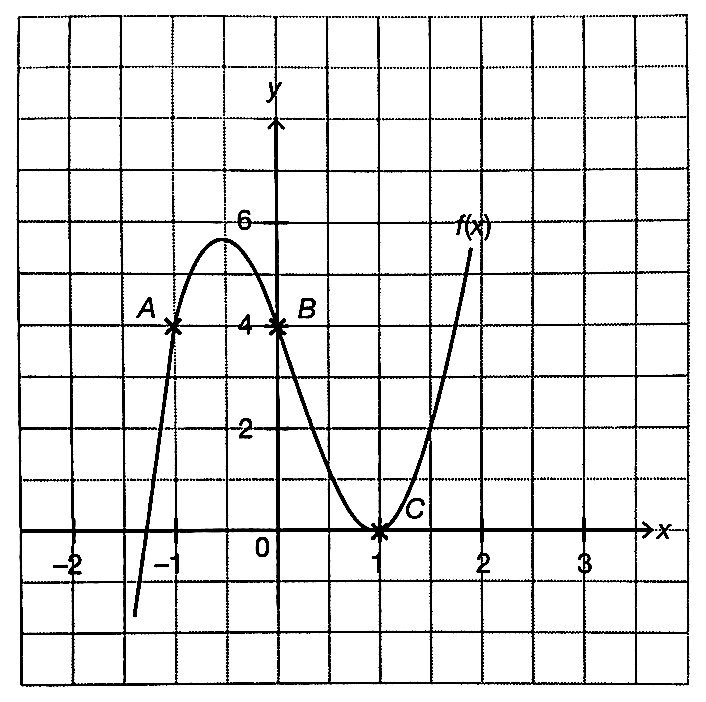
\includegraphics[width=0.3\textwidth]{./images/q24.jpeg}
                  \end{center}
                  \begin{enumerate}
                        \item Find the gradient function of the tangent to the curve $f(x)$.
                        \item \begin{enumerate}
                                    \item Find the values of gradient of the tangents to the curve at points $A$, $B$,
                                          and $C$.
                                    \item Hence, elaborate the situations of the tangents at points $A$, $B$, and $C$
                                          based on the values of the gradient obtained in (i).
                              \end{enumerate}
                  \end{enumerate}
            \item Find the gradient of the tangent for each of the following curves at the given
                  point $P$.
                  \begin{enumerate}
                        \item $y = 4x - \dfrac{8}{x}; P(4, 14)$
                        \item $y = \dfrac{4 - 3x^2}{3-2x}; P(2, 8)$
                  \end{enumerate}
            \item \begin{enumerate}
                        \item Find the value of gradient of the tangent to the curve $y = 2x^3 - 3x^2$ when
                              $x = 1$.
                        \item Find the coordinates of points to the curve $y = \dfrac{x^3}{3} + x^2 - 1$ such
                              that the gradient to the curve at the points is $8$.
                        \item Given the curve $y = ax^2 + bx + 3$ has the gradient $5$ when $x = 2$ and the
                              gradient $0$ when $x = -3$. Determine the values of $a$ and $b$.
                  \end{enumerate}
            \item Find the equations of tangent and normal to the curve $y = 8 - 2x - x^2$ at
                  each of the following points.
                  \begin{enumerate}
                        \item $A(1, 5)$
                        \item $C(-1, 9)$
                  \end{enumerate}
            \item \begin{enumerate}
                        \item Find the equation of normal to the curve $y = 3x^2 + 8x - 7$ at point $(-2,
                                    6)$.
                        \item Given the tangent to the curve $y = ax^2 + bx$ at the point $P(4, 8)$ is
                              perpendicular to the straight line that passes through the point $A(4, 1)$ and
                              the point $B(12, 0)$. Find the values of $a$ and $b$.
                  \end{enumerate}
            \item A curve $y_1 = x^2 - x - 5$ intersects another curve $y_2 = x^2 -
                        \dfrac{31}{5}x + \dfrac{53}{5}$ at point $A$.
                  \begin{enumerate}
                        \item Determine the gradient functions for both curves at the point of intersection
                              $A$.
                        \item Show that the tangents of both curves at point $A$ are normal to each other.
                  \end{enumerate}
            \item Given the equation of a normal for a curve $y = x^2 + 2x - 5$ at point $A(2,
                        3)$ is given bt $y = ax + b$. Find the values of $a$ and $b$.
      \end{enumerate}
      \subsection{Turning Points, Concavity, and Stationary Points}
      \begin{enumerate}
            \item Find the coordinates of the turning points for each of the following curves.
                  Hence, determine the nature of the turning points.
                  \begin{enumerate}
                        \item $y = 5x^2 - 2x + 1$
                        \item $y = \dfrac{x^2}{x+1}$
                        \item $y = 7 - x^3$
                  \end{enumerate}
            \item The following diagram shows the plan of a cuboid in which its centre in the
                  shape of a cylinder is taken out. The cuboid measures $3x\textit{cm} \times
                        2x\textit{cm} \times (45 - 5x)\textit{cm}$.
                  \begin{center}
                        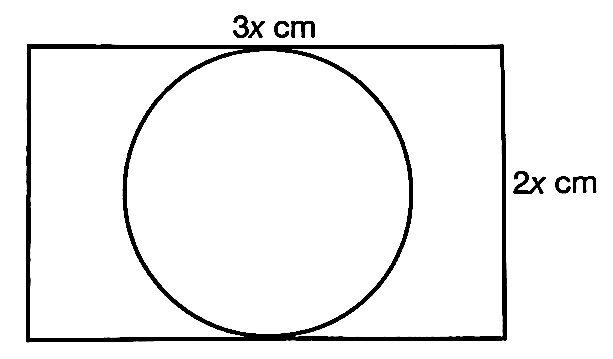
\includegraphics[width=0.3\textwidth]{./images/q30.jpeg}
                  \end{center}
                  Find the value of $x$ that makes the volume of the cylinder taken out a maximum.
            \item Given $A = bh$ where $b^2 + h^2 = 40$ and $b, h > 0$. Find the values of $b$
                  and $h$ so that $A$ becomes a stationary point and show that the value of $A$
                  is maximum.
            \item A piece of wire with a length of $120\textit{cm}$ is divided into two parts
                  where is each is bent to form an equilateral triangle with an edge of
                  $x\textit{cm}$ and a square with an edge of $y\textit{cm}$ respectively.
                  Express $y$ in terms of $x$. Hence, show that the total area of both shapes,
                  $A\textit{cm}^2$ is given by
                  \[A = \dfrac{9{(40 - x)}^2 + 4\sqrt{3}x^2}{16}\]
                  Calculate the value of $x$ so that $A$ has a stationary value. Determine
                  whether this value of $x$ makes $A$ a maximum of a minimum.
            \item Chan wants to build two separate pens by using a fence of $100\textit{m}$. Both
                  pens are square in shape.
                  \begin{center}
                        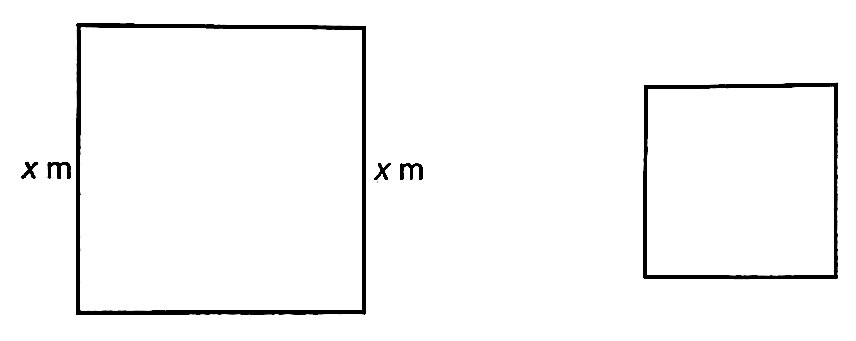
\includegraphics[width=0.4\textwidth]{./images/q30_2.jpeg}
                  \end{center}
                  If the edge of the larger pen is $x\textit{m}$,
                  \begin{enumerate}
                        \item find the length of the side of the smaller pen in terms of $x$.
                        \item find the value of $x$ such that the total area of both pens is minimum.
                  \end{enumerate}
            \item A factory needs to produce containers of the same size for a type of breakfast
                  cereals as shown in the diagram below. Each container must have a volume of
                  $2666\dfrac{2}{3}\textit{cm}^3$. The base of the containers is rectangular in
                  shape with its length twice the width. In order to reduce the production cost,
                  the total surface area of each container must be minimum.
                  \begin{center}
                        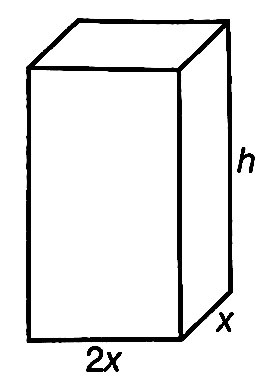
\includegraphics[width=0.15\textwidth]{./images/k2q7.jpeg}
                  \end{center}
                  \begin{enumerate}
                        \item Find the dimensions of the containers produced.
                        \item Hence, find the total cost of production for $20000$ units of containers if the
                              cost of production for a containers is RM$0.002$ per $\textit{cm}^2$.
                  \end{enumerate}
            \item An opened right circular cone with the base radius $r\textit{cm}$ and slant
                  height $12\textit{cm}$ is used to cover a ball with radius $j\textit{cm}$ such
                  that the ball is inscribed in the cone as shown in the cross-section diagram
                  below.
                  \begin{center}
                        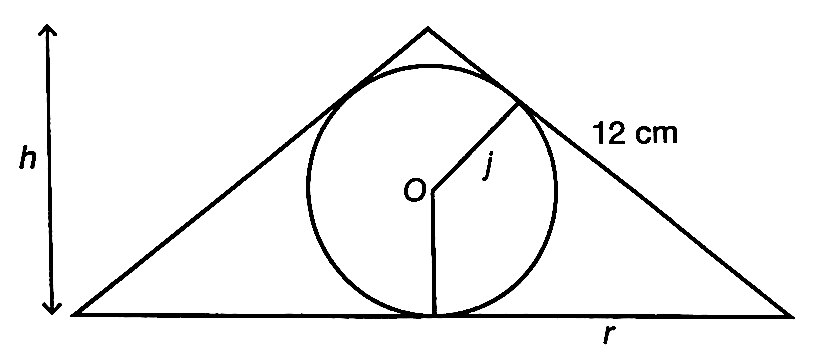
\includegraphics[width=0.35\textwidth]{./images/k2q8.jpeg}
                  \end{center}
                  Show that the volume of the cone is given by $V = \dfrac{\pi}{3}(144h - h^3)$.
                  Hence, determine the dimensions of the right circular cone such that its volume
                  is maximum and find the radius of the ball, $j$, which corresponded to the
                  maximum volume of the cone.
      \end{enumerate}
      \subsection{Rates of Change}
      \begin{enumerate}
            \item The total surface area, $A\textit{cm}^2$, of a metal solid which consists of a
                  cone and a cylinder with a common radius, $r\textit{cm}$ is given by $A =
                        2\pi\left(\dfrac{18}{r} + \dfrac{r^2}{3}\right)$. When it is heated, its total
                  surface area changes at the rate of $2.1\pi \textit{cm}^2\textit{s}^{-1}$. Find
                  the rate of change of the radius, in $\textit{cm} \textit{s}^{-1}$, at the
                  instant $r = 6\textit{cm}$.
            \item A spherical balloon experiences a constant rate of increase of
                  $6\textit{cm}^2\textit{s}^{-1}$.
                  \begin{center}
                        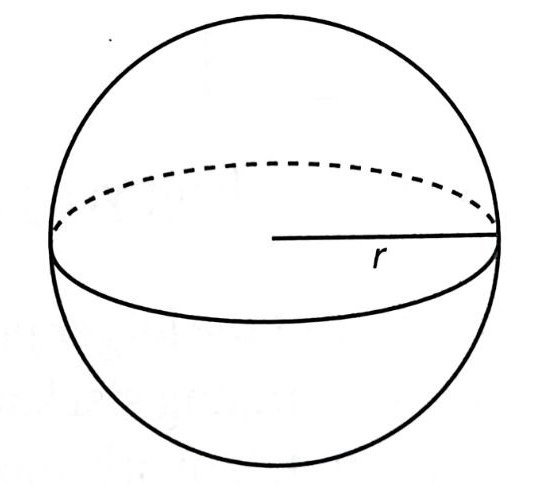
\includegraphics[width=0.3\textwidth]{./images/q31.jpeg}
                  \end{center}
                  At the instant when the radius is 5\textit{cm}, find
                  \begin{enumerate}
                        \item the rate of increase, in $\textit{cm} \textit{s}^{-1}$, of the radius.
                        \item the rate of increase if volume, in $\textit{cm}^3 \textit{s}^{-1}$, of the
                              sphere.
                  \end{enumerate}
            \item The following diagram shows a container in the shape of a cone. Given its
                  height is equal to its base radius. Water is poured into the container at the
                  rate of $80\textit{cm}^3\textit{s}^{-1}$. The volume of the water in the
                  container is $\dfrac{1}{3}\pi x^3\textit{cm}^3$, when the depth of the water is
                  $x\textit{cm}$.
                  \begin{center}
                        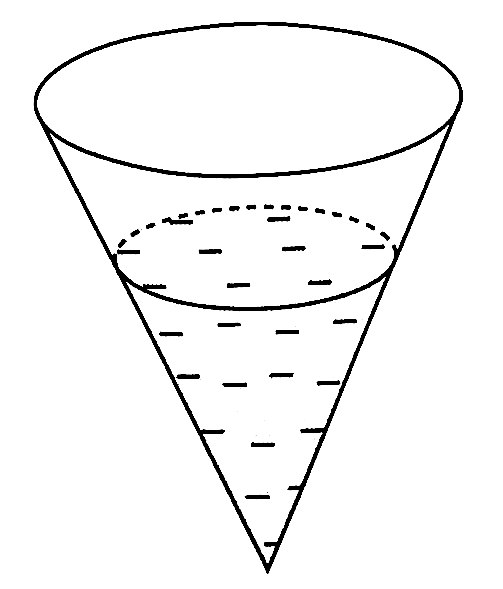
\includegraphics[width=0.2\textwidth]{./images/q31_2.jpeg}
                  \end{center}
                  Calculate, at the instant when the depth of the water is $10\textit{cm}$,
                  \begin{enumerate}
                        \item the rate of increase of the depth, in $\textit{cm} \textit{s}^{-1}$, of the
                              water.
                        \item the rate of increase of the horizontal surface area, in $\textit{cm}^2
                                    \textit{s}^{-1}$, of the water.
                  \end{enumerate}
            \item A hemispherical bowl of radius $R\textit{cm}$ is filled with water to a depth
                  of $h\textit{cm}$.
                  \begin{center}
                        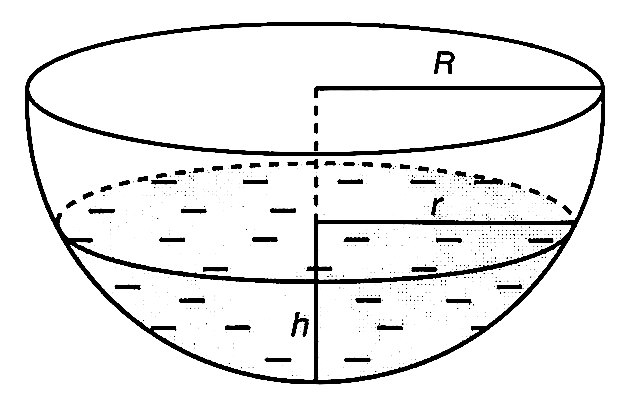
\includegraphics[width=0.3\textwidth]{./images/q33.jpeg}
                  \end{center}
                  The volume of the water in the bowl is given by $V = \dfrac{\pi}{3}(3Rh^2 - h^3)$.
                  \begin{enumerate}
                        \item Show that the radius of the water surface, $r$, is given by $r = \sqrt{2Rh -
                                          h^2}$.
                        \item Water is poured into the bowl at a constant rate of
                              $300\textit{cm}^3\textit{min}^{-1}$. Find, in terms of $R$, the rate of
                              increase of the surface area, in $\textit{cm}^2 \textit{min}^{-1}$, of the
                              water when $2h = R$.
                  \end{enumerate}
            \item A wire of length of $26\textit{cm}$ is bent to form a sector with centre $O$
                  and radius $r\textit{cm}$ as in the diagram below.
                  \begin{center}
                        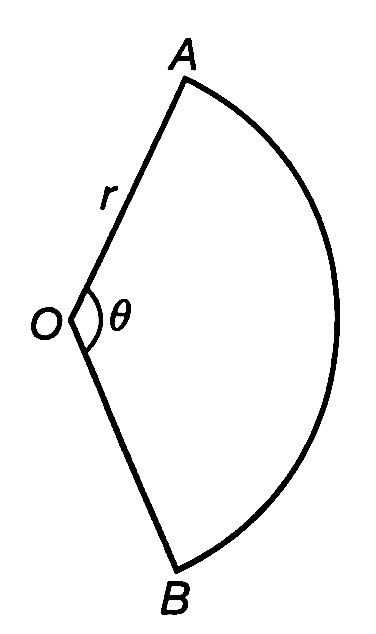
\includegraphics[width=0.15\textwidth]{./images/k2q6.jpeg}
                  \end{center}
                  \begin{enumerate}
                        \item Express $\theta$ in terms of $r$.
                        \item If the radius increases at the rate of $0.1\textit{cm}\textit{s}^{-1}$, find,
                              at the instant $r = 2\textit{cm}$,
                              \begin{enumerate}
                                    \item the rate of change, in $\textit{rad}\textit{s}^{-1}$, of $\theta$.
                                    \item the rate of change of the area, in $\textit{cm}^2\textit{s}^{-1}$, of the
                                          sector.
                              \end{enumerate}
                  \end{enumerate}
      \end{enumerate}
      \subsection{Small Changes and Approximations}
      \begin{enumerate}
            \item Given that $y = 2x^3 - 5x^2 + x - 1$, find the value of $\dfrac{dy}{dx}$ when
                  $x = 1$. Hence, find the small changes in $y$ when $x$ increases from $1$ to
                  $1.02$.
            \item Given the equation of a curve is $y = \dfrac{9}{{(2x - 5)}^2}$, find, in terms
                  of $p$, where $p$ is a small value, the approximate change in
                  \begin{enumerate}
                        \item $y$ when $x$ increases from $3$ to $3 + p$.
                        \item $x$ when $y$ decreases from $1$ to $1 - p$.
                  \end{enumerate}
            \item Given $y = x^4$, by using the calculus method, find the approximate value of
                  \begin{enumerate}
                        \item $2.03^4$.
                        \item $1.99^4$.
                  \end{enumerate}
            \item Given the equation of a curve $y = 2x^3 + x$. By using the differentiation
                  method, find in terms of $p$, the approximate percentage increase in $y$ when
                  $x$ increases from $2$ by $p\%$, where $p$ is a small value.
            \item By using the calculus method, show the steps to determine the value of
                  $9.02^{-\frac{1}{2}}$.
            \item Diagram below shows a metal solid with a uniform cross-section in the shape of
                  a right trapezium $PQRS$.
                  \begin{center}
                        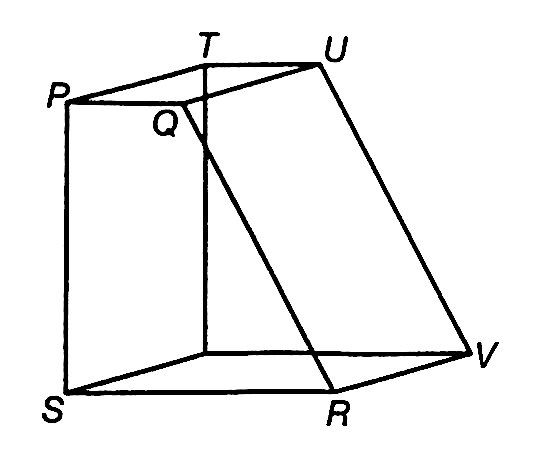
\includegraphics[width=0.25\textwidth]{./images/k2q5.jpeg}
                  \end{center}
                  Given that $PQ$ is $x\textit{cm}$, $PQ:PS:SR = 2:5:3$ and the area of its
                  cross-section is $A\textit{cm}^2$.
                  \begin{enumerate}
                        \item Express $A$ in terms of $x$.
                        \item \begin{enumerate}
                                    \item When the metal is heated, $x$ increases at the rate of
                                          $0.02\textit{cm}\textit{s}^{-1}$. Find the rate of change of the area, in
                                          $\textit{cm}^2\textit{s}^{-1}$, of the cross-section when $x = 4\textit{cm}$.
                                    \item Given the thickness of the metal is $\dfrac{2}{5}x\textit{cm}$, find the
                                          approximate change of the volume, in $\textit{cm}^3$, of the metal when $x$
                                          changes from $4\textit{cm}$ to $4.05\textit{cm}$.
                              \end{enumerate}
                  \end{enumerate}
      \end{enumerate}
\end{multicols}
\end{document}